\documentclass[11pt]{article}

\usepackage{color}
\usepackage[usenames,dvipsnames,svgnames,table]{xcolor}

\usepackage{graphicx}
\usepackage{amsmath}
\usepackage{amssymb}
\usepackage{eulervm}
\usepackage{charter}
\usepackage{exercise}
\PassOptionsToPackage{hyphens}{url}\usepackage{hyperref}
\hypersetup{colorlinks=true,linkcolor=DarkRed,urlcolor=DarkRed}
\usepackage{float}
\usepackage{enumitem}
\usepackage{bm}

\newcommand{\p}{\;\text{.}}

\newcommand{\R}{{\mathbb R}}
\newcommand{\N}{{\mathbb N}}
\newcommand{\E}{{\mathbb E}}

\newcommand{\U}{{\bm U}}
\newcommand{\V}{{\bm V}}
\newcommand{\W}{{\bm W}}
\newcommand{\A}{{\bm A}}
\newcommand{\B}{{\bm B}}
\newcommand{\C}{{\bm C}}
\newcommand{\ba}{{\bm a}}
\newcommand{\bb}{{\bm b}}
\newcommand{\boc}{{\bm c}}
\newcommand{\bu}{{\bm u}}
\newcommand{\bv}{{\bm v}}
\newcommand{\bw}{{\bm w}}
\newcommand{\x}{{\bm x}}
\newcommand{\y}{{\bm y}}
\newcommand{\z}{{\bm z}}
\newcommand{\X}{{\bm X}}
\newcommand{\Y}{{\bm Y}}
\newcommand{\Z}{{\bm Z}}
\newcommand{\bt}{{\bm t}}
\newcommand{\ma}[1]{\begin{pmatrix}#1\end{pmatrix}}

\DeclareMathOperator*{\argmin}{arg\,min}
\DeclareMathOperator*{\argmax}{arg\,max}

\newcommand{\ans}[2]{{\leavevmode\color{OliveGreen}#2}} % no answers
% \newcommand{\ans}[2]{{\leavevmode\color{OliveGreen}#1}} % answers

\newcommand{\red}[1]{{\textcolor{Red}{#1}}}
\definecolor{myred}{HTML}{C82506}
\definecolor{myblue}{HTML}{0365C0}
\definecolor{mygreen}{HTML}{00882B}
\definecolor{myorange}{HTML}{DE6A10}
\definecolor{mypurple}{HTML}{773F9B}
\definecolor{myyellow}{HTML}{DCBD23}

\newcommand{\rc}[1]{{\textcolor{myred}{ #1 }}}
\newcommand{\gc}[1]{{\textcolor{mygreen}{ #1 }}}
\newcommand{\bc}[1]{{\textcolor{myblue}{ #1 }}}
\newcommand{\kc}[1]{{\textcolor{Gray}{ #1 }}}
\newcommand{\oc}[1]{{\textcolor{myorange}{ #1 }}}
\newcommand{\pc}[1]{{\textcolor{mypurple}{ #1 }}}
\newcommand{\yc}[1]{{\textcolor{myyellow}{ #1 }}}

\newcommand{\kp}{{\kc{\partial}}}
% Exam questions
\newcommand{\trueorfalse}{\linebreak \textbf{A } True ~~ \textbf{B } False}
\newcommand{\choices}[4]{\linebreak\noindent\textbf{A } #1~~\textbf{B } #2~~\textbf{C } #3~~\textbf{D } #4}
%\newcommand{\choicesnum}[4]{\linebreak\noindent{\fill}\textbf{A } \np{#1}~~\textbf{B } \np{#2}~~\textbf{C } \np{#3}~~\textbf{D } \np{#4}}
%\newcommand{\twochoices}[2]{\linebreak\noindent\textbf{A } #1~~\textbf{B } #2}
%\newcommand{\threechoices}[3]{\linebreak\noinden\textbf{A } #1~~\textbf{B } #2~~\textbf{C } #3}
\newcommand{\choicesv}[4]{\\ \begin{minipage}{\textwidth}\vspace{4pt}\noindent\textbf{A } #1\\ \noindent\textbf{B } #2\\ \noindent\textbf{C } #3\\ \noindent\textbf{D } #4\end{minipage}}

% Homework questions
\newcommand{\qu}[0]{%
  \addtocounter{Question}{1}%
  \noindent \textbf{question \theQuestion:}
}


\newcommand{\an}{\ans{\checkmark}{}}

%\usepackage{tikz}
%\usepackage{tikz-qtree}
\usepackage{qtree}
\usepackage{xfrac}
\usepackage{graphicx}

\title{Week 5: Support Vector Machines\\ and Tensor Backpropagation}

\begin{document}
\author{\url{https://mlvu.github.io}}

\maketitle

\section{Support Vector Machines}

\subsection{Tensor loss}

The basic optimization objective for Support Vector Machines is 
\begin{align*}
\text{minimize}\;\;&\frac{1}{2}||\oc{\bw}|| + \rc{C}\sum_i \gc{p_i}\\
\text{such that}\;\;&y_i(\oc{\bw}^T\x_i + \bc{b}) \geq 1 - \gc{p_i}\\
\text{and} \;\;&\gc{p_i} \geq 0
\end{align*}

\qu What does $i$ index? How many terms does the sum have, and how many constraints are there?

\ans{It iterates over the data. There are as many terms as there are instances in the data. There are two constraints per instance.}{}

What is the value of $y_i$ in this expression? What is its function?

\ans{$y_i$ is 1 for positive examples, and -1 for negative examples. It allows us to rewrite the constraints

\begin{align*}
\oc{\bw}^T\x_i + \bc{b} \geq 1 &\;\text{if $\x_i$ is positive} \\	
\oc{\bw}^T\x_i + \bc{b} \leq -1 &\;\text{if $\x_i$ is negative} \\
\end{align*}

to a single constraint.
}{}


\qu There are two common ways to rewrite this expression before implementing it. What are they (in general terms) and what are their benefits?

\ans{The first option is to rewrite everything in terms of $\bw$ and $b$ in order to get rid of the constraints. This is useful when we want to use the SVM as the last layer in a neural network. Without constraints, we are free to use basic backpropagation.

The second option is to use Lagrange multipliers to get rid of $\oc{\bw}$ and rewrite everything in terms of the multipliers. This expresses the solution purely in terms of the support vectors.

The main benefit is that the whole algorithm can be written in terms of the dot products of pairs of instances. This means we do not need to see the actual feature vectors to compute the support vectors, only the dot products. This allows us to apply the \emph{kernel trick}.
}{}

\subsection{Lagrange multipliers} 


Lagrange multipliers are a useful trick to know. In the lectures we only had time to describe the trick itself, and the rules for applying it. That should be enough to do the exam questions and the questions below, but if you want some more intuition for why Lagrange multipliers work the way they do please read  \href{https://www.khanacademy.org/math/multivariable-calculus/applications-of-multivariable-derivatives/constrained-optimization/a/lagrange-multipliers-single-constraint}{this article from the required reading}.

We have the following optimization problem:
\begin{align*}
\text{minize} &\;f(\bc{a}, \bc{b}) = \bc{a}^2 + 2\bc{b}^2 \\
\text{such that} &\;\bc{a}^2 = - \bc{b}^2 + 1
\end{align*}


\qu The first step is to rewrite the constraint so that the right side is equal to zero. Do so.
\ans{$\bc{a}^2 + \bc{b}^2 - 1 = 0$}{}
What does the constraint say about the allowed inputs (what shape do the allowed inputs make in the $(\bc{a}, \bc{b})$-plane)?
\ans{The solutions are constrained to a circle, centered on the origin, with radius 1 (the so-called bi-unit circle).}{}


We now define a function $L(\bc{a}, \bc{b}, \rc{\alpha}) = f(\bc{a}, \bc{b}) + \rc{\alpha} G$, where $G$ is the left hand side of the constraint equal to zero (how much any given $a$ and $b$ violate the constraint).\footnotemark 

\qu Write out $L(\bc{a}, \bc{b}, \rc{\alpha})$ for our problem.
\ans{$L(\bc{a}, \bc{b}, \rc{\alpha}) = \bc{a}^2 + 2\bc{b}^2 + \alpha(\bc{a}^2 + \bc{b}^2 - 1) $}{}	

\footnotetext{For plain Lagrange multipliers, where the constraints are all equalities, we can either add or subtract the term containing the constraint. For inequality constrains, it depends on whether we are maximizing or minimizing.}

We take the derivative of $L$ with respect to each of its \emph{three} parameters, and set these equal to zero. 

\qu Fill in the blanks
\ans{
\begin{align*}
\frac{\kp L}{\kp \bc{a}} &= \frac{\kp(\bc{a}^2 + 2\bc{b}^2 + \rc{\alpha} \bc{a}^2 + \rc{\alpha} \bc{b}^2 - \rc{\alpha})}{\kp \bc{a}} \\
&= 2\bc{a} + 2\rc{\alpha} \bc{a} \\
 	\frac{\kp L}{\kp \bc{b}} &= 4\bc{b} + 2 \rc{\alpha} \bc{b} \\
 	\frac{\kp L}{\kp \rc{\alpha}} &= \bc{a}^2 + \bc{b}^2 - 1 
\end{align*}
}{}

\begin{align}
a (\ans{2+2\rc{\alpha}}{\ldots})&= 0\\
b (\ans{4 + 2\rc{\alpha}}{\ldots})&= 0 \\
a^2 + b^2 &= 1 \label{line:constraint}
\end{align}

\noindent Note that the last line recovers the original constraint. We now have three equations with three unknowns, so we can solve for $a$ and $b$. From the shape of the function (it's symmetric in both the $a$ and $b$ axes), we should expect at least two solutions. 

We can get these from the above equations by noting that if $\bc{a}$ and $\bc{b}$ are both nonzero, we can derive a contradiction. Thus either $\bc{a}$ or $\bc{b}$ must be zero.

\qu Give the solutions for both cases (remember that $x^2 = 1$ has \emph{two} solutions).

\ans{
From line (\ref{line:constraint}), above we see that if $a =0$, then $b^2=1$ and vice versa. This gives us
\begin{align*}
a = 0&, b = 1\\	
a = 0&, b = -1\\
a = 1&, b = 0\\
a = -1&, b = 0\\
\end{align*}
as extrema. Filling these in, we find that the last two lines minimize the function. (The first two are maxima, as can be seen by clicking the Wolfram Alpha link below.
}{}

Happily, \href{https://goo.gl/Uaz5mg}{Wolfram Alpha} agrees with us (and provides some informative plots).

\subsection{The kernel trick}

The feature space of $\oc{k}$ is a projection of point $\ba$ to point $\ba'$ such that 
\[
\oc{k}(\ba, \bb) = {\ba'}^T\bb' \p
\]

We have a dataset with two features Let $\bm{a} = \ma{a_1\\ a_2}$ and $\bm{b} = \ma{b_1\\ b_2}$. We define the \emph{kernel}
\[
\oc{k_1}(\bm{a}, \bm{b}) = (\bm{a}^T\bm{b})^2 \p
\]

\qu Show that the feature space defined by$\oc{k_!}$ is 
\[ 
\ma{{x_1}^2\\\sqrt{2}x_1x_2\\{x_2}^2}\p
\]
Hint: start by writing out the definition as a scalar function. See if you can re-arrange this back into a dot procut of two other vectors.
\ans{


Starting from the definition of $k$:
\begin{align*}
k(\ba, \bb) &= \left( \ma{a_1\\ a_2}^T\ma{b_1\\ b_2} \right)^2\\
 &= \left ( a_1 b_1 + a_2 b_2 \right)^2 \\
 &= a_1 b_1 a_1 b_1 + 2 a_2 b_2 a_1 b_1 + a_2 b_2 a_2 b_2 \\
 &= a_ 1a_1\cdot b_1 b_1 + 2 \cdot a_1 a_2 \cdot b_1 b_2 + a_2a_2\cdot b_2b_2\\
 &= \ma{a_1a_1\\ \sqrt{2}a_1a_2\\a_2a_2} ^T \ma{b_1b_1\\ \sqrt{2}b_1b_2\\b_2b_2}
\end{align*}
}{}
	
\qu What is the feature space for the kernel
\[
\oc{k_2}(\ba, \bb) = \left(\ba^T\bb +1\right)^2\;\;\;\text{?}
\]
\ans{
\begin{align*}
k(\ba, \bb) &= \left( \ma{a_1\\ a_2}^T\ma{b_1\\ b2} + 1\right)^2\\
 &= (a_1 b_1 + a_2 b_2)^2 +  2( a_1 b_1 + a_2 b_2) + 1 \\
 &= a_1b_1a_1b_1 + 2a_1b_1a_2b_2 + a_2b_2a_2b_2 + 2a_1b_1 + 2a_2b_2 + 1\\
 &= \ma{1 \\ \sqrt{2}a_1 \\ \sqrt{2}a_2 \\ {a_1}^2\\\sqrt{2}a_1a_2 \\{a_2}^2} ^T\ma{1 \\ \sqrt{2}b_1 \\ \sqrt{2}b_2 \\ {b_1}^2\\\sqrt{2}b_1b_2 \\{b_2}^2} 
\end{align*}
}{}

\section{Backpropagation Revisited}

\subsection{The multivariate chain rule}

If we want to do backpropagation for a computation graph where an output variable depend in an input variable through multiple intermediate values (the graph contains a diamond), we require the \emph{multivariate chain rule}. If you don't quite remember how it goes, re-read slides 24--29 fo the deep learning lecture before trying these questions.


We will use the backpropagation algorithm to find the derivative of the function
\[
f(x) = \sin(x^2)\cos(x^3)
\]
with respect to $x$.

\qu First, we break the function up into modules. Fill in the blanks.

\begin{align*}
f &= \rc{a}\gc{b} \\
\rc{a} &= \ans{\sin(c)}{\ldots}\\
\gc{b} &= \ans{\cos(d)}{\ldots} \\
\oc{c} &= x^2 \\
\bc{d} &= x^3 \\
\end{align*}

\qu Draw the computation graph with nodes $x, \oc{c}, \bc{s}, \rc{a}, \gc{b}, f$

\ans{

\hspace{5em}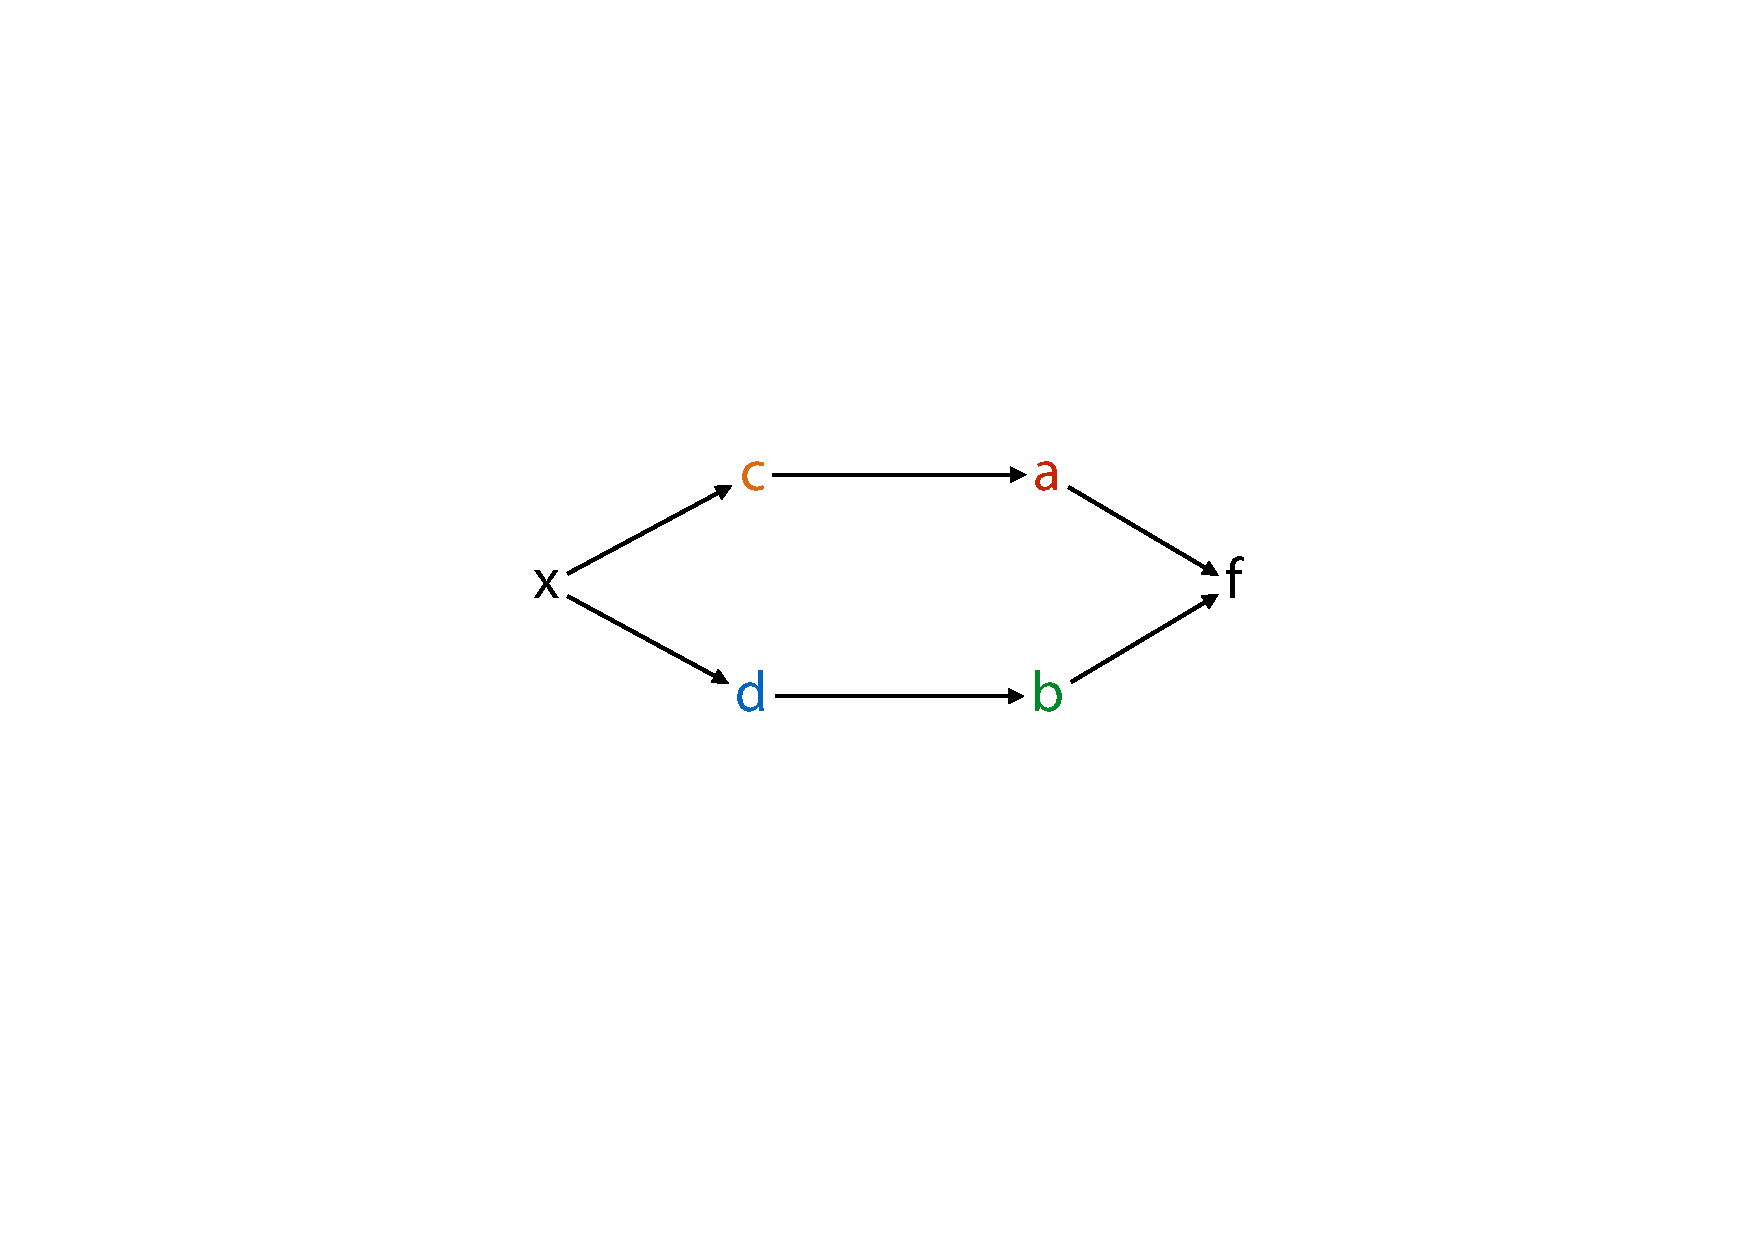
\includegraphics[width=0.4\linewidth]{compgraph}

}{}

\qu Work out the \emph{local} derivatives. Which is the correct expression for the gradient $\kp f / \kp x$?

\ans{
\begin{align*}
\frac{\kp f}{\kp x} &= \frac{\kp f}{\kp \rc{a}}\frac{\kp \rc{a}}{\kp x} + \frac{\kp f}{\kp \gc{b}}\frac{\kp \gc{b}}{\kp x} & \text{multivariate chain rule}\\
&= \frac{\kp f}{\kp \rc{a}} \frac{\kp \rc{a}}{\kp \oc{c}} \frac{\kp \oc{c}}{\kp x} + \frac{\kp f}{\kp \gc{b}}\frac{\kp \gc{b}}{\kp x} & \text{chain rule for $\oc{c}$: $\frac{\rc{a}}{x} = \frac{\kp \rc{a}}{\kp \oc{c}} \frac{\kp \oc{c}}{\kp x}$}\\
&= \frac{\kp f}{\kp \rc{a}} \frac{\kp \rc{a}}{\kp \oc{c}} \frac{\kp \oc{c}}{\kp x} + \frac{\kp f}{\kp \gc{b}}\frac{\kp \gc{b}}{\kp \bc{d}}\frac{\bc{d}}{x} & \text{chain rule for $\bc{d}$}\\
 &= \gc{b} \cdot \cos(\oc{c}) \cdot 2x - \rc{a}\cdot \sin(\bc{d})\cdot 3x^2& \text{work out all local derivatives}
\end{align*}}{}

\noindent This is a common exam question so make sure to practice if you're not sure. You can easily create new questions for yourself by coming up with any function $f(x)$ with a diamond shape in the computation (just make sure that $x$ is used twice).

\subsection{Tensor Backpropagation}

In scalar backpropagtion, we need to work out only the local derivatives. Once we have these, we can multiply them in any order to get the global derivative. If we want to apply backpropagation to tensors, things are not so easy.

\qu Why not? What is it about the local derivatives in tensor backpropagation that makes it difficult to apply in this way?

\ans{In tensor backpropagation, the local derivatives are often, for instance, the derivative of a vector function over matrix parameters, like the local derivative $\kp \gc{\bm k}/\kp \oc{\bm W}$ shown in the slides. In this case, the collection of all scalar derivatives (every output with every input) is best represented as a 3 tensor. This would take way too much memory, and there's then no natural way to multiply this local derivative with the others to compute the global derivative.}{}

The solution is not to compute the local derivatives explicitly, but only to compute the gradients on the inputs over the loss, given the gradients of the outputs over the loss. 

We will practice this for a simple feedforward layer (without activation). Consider a module $f$ that computes:\footnotemark
\[
\y = f(\x, \oc{\W}, \bc{\bb}) = \oc{\W}\x + \bc{\bb}
\]

\footnotetext{Normally, we would consider $\x$ the input, and $\oc{\W}$ and $\bc{\bb}$ the parameters, but for our AD engine, the distinction does not matter: everything going in to the computation is an input, and we may need the gradient over all three.}

\noindent Assume that this module is part of a much larger network. Its output $\y$ is fed as input to another module, which produces a new output that is fed to another module and so on. At the end, a single scalar loss $L$ is produced.

\hspace{5em}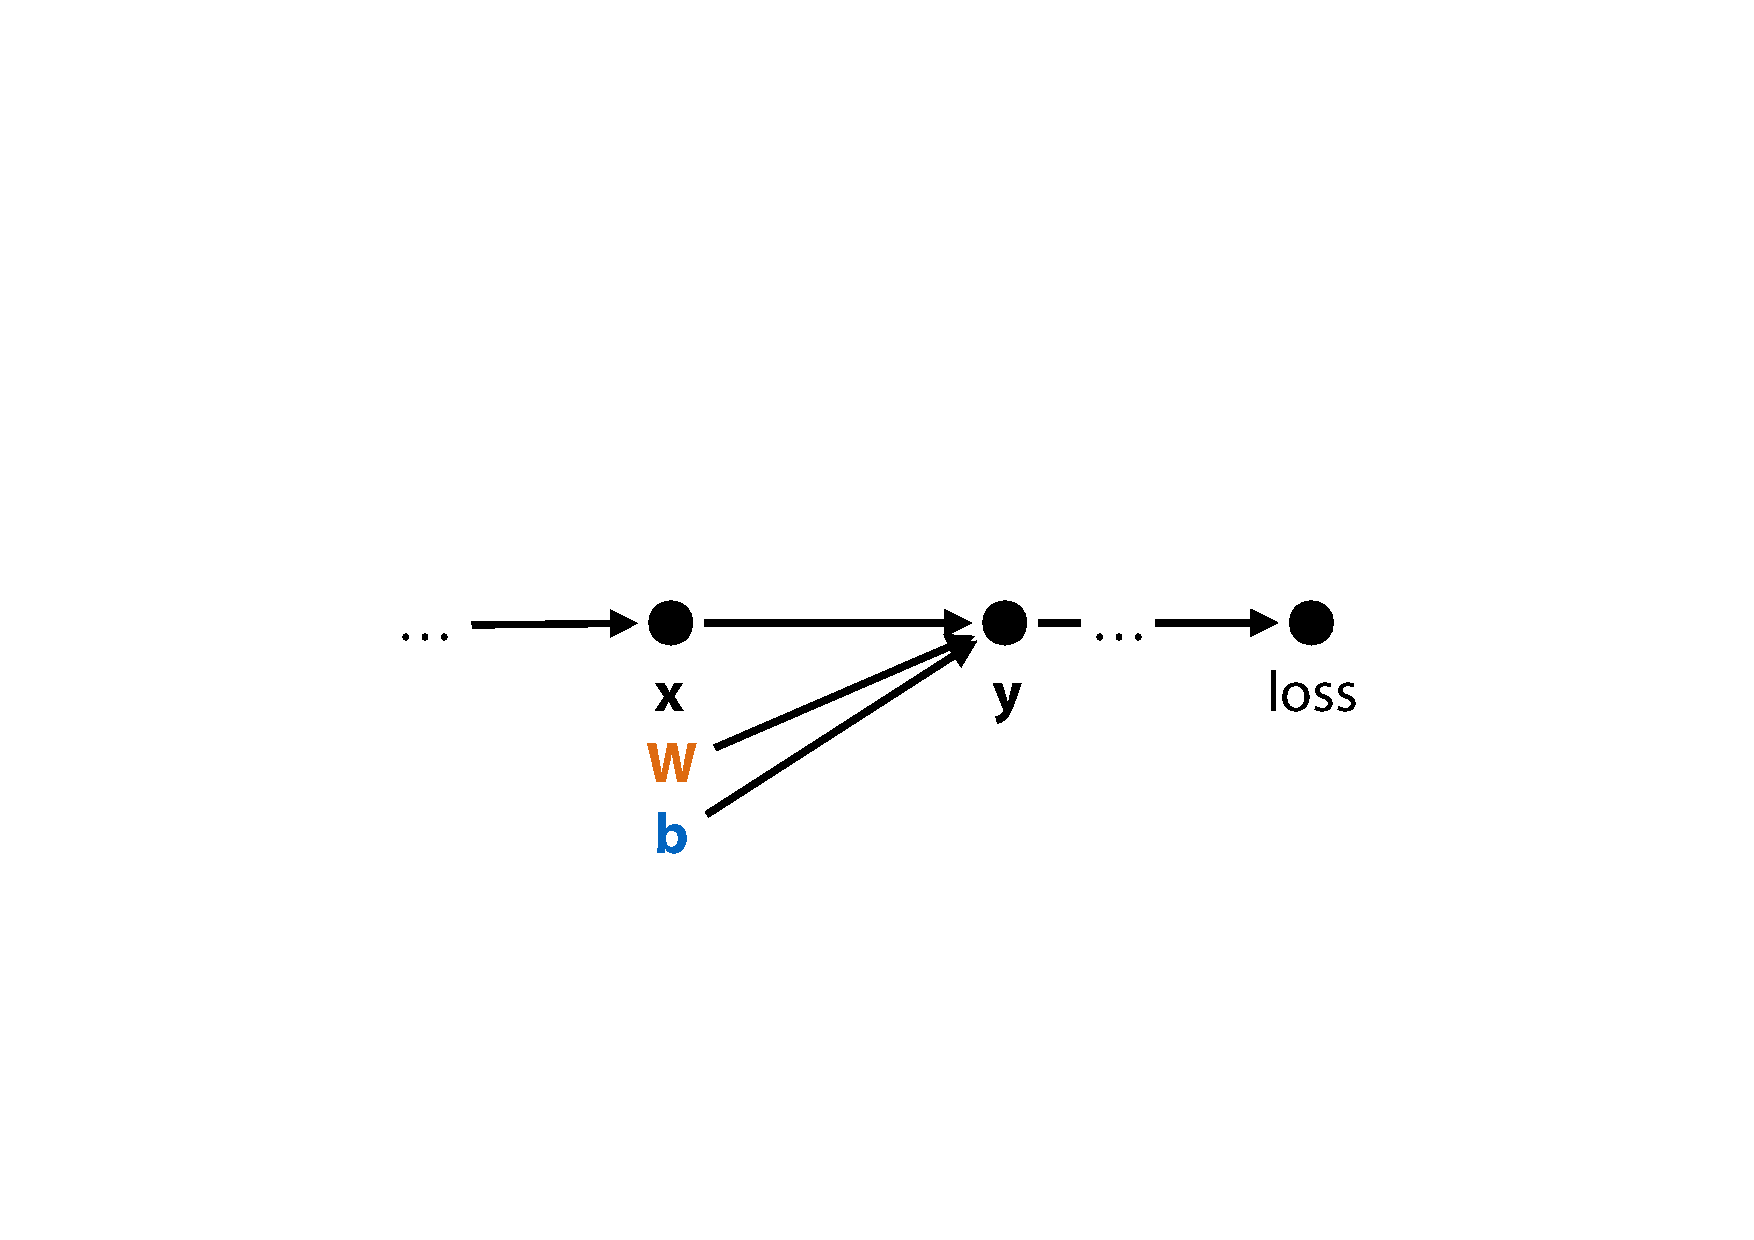
\includegraphics[width=0.7\linewidth]{networkloss}
 
\noindent Ultimately, we want to work out the derivative of this loss,  with respect to our inputs:
\[
\frac{\kp L}{\kp \x}\;\;\; \frac{\kp L}{\kp \oc{\W}}\;\;\; \frac{\kp L}{\kp \bc{\bb}}
\]


\noindent We'll start with the bias term $\bc{\bb}$. Since matrix/vector calculus can get complicated, and doesn't translate to tensors of higher rank, we'll develop everything in terms of scalar calculus.  Once we've taken the derivatives we'll transform everything to matrix operations to make the implementation efficient.

We're interested in $\frac{\kp L}{\y}\frac{\kp \y}{\kp \bc{b}_j}$, but we need matrix/vector calculus to do that. Instead we will consider $L(f(\bc{\bb}))$ as a \emph{scalar} computation, which has multiple intermediate values $y_1, y_2 \ldots, y_k$. By the multivariate chain rule, we can just take the derivative over each path (through each value $y_i$), and sum them:
\[
\frac{\kp L}{\kp \bc{b}_j} = \sum_i \frac{\kp L}{\kp y_i} \frac{\kp y_i}{\kp \bc{b}_j}
\]

\noindent We will assume that $\kp L/\kp y_i$ is given to us by the AD engine as a vector $\bm d$ with $d_i = \kp L/\kp y_i$. All we need to work out is a simple matrix operation that computes $\kp L/\kp \bc{b}_j$ for all $j$ and lays the results out in the same shape as $\bc{\bb}$. We'll start by working out the scalar derivative.


\qu Fill in the gaps
\begin{align*}
\frac{\kp L}{\kp \bc{b}_j} &= \sum_i \frac{\kp L}{\kp y_i} \frac{\kp y_i}{\kp \bc{b}_j} = \sum_i d_i \ans{\frac{\kp y_i}{\kp \bc{b}_j}}{\ldots}\\
&= \sum_i d_i \frac{\kp [\ans{\oc{\W}\x + \bc{\bb}}{\ldots}]_i}{\kp \bc{b_j}} = \sum_i d_i \frac{\kp [\oc{\W}\x]_i + \bc{b}_i}{\kp \bc{b_j}}\\
&= \sum_i d_i\frac{\kp \bc{b}_i}{\kp \bc{b}_j} = \ans{d_j}{\ldots}
\end{align*}

\qu What should the \texttt{backward()} function for $f$ return as the gradient of $\bc{\bb}$?

\ans{We should return a vector $\bc{\bb}'$ with the same shape as $\bc{\bb}$, where $\bc{b}'_j = \kp L / \kp \bc{b}_j$. Since $d_j$ is the gradient for $\bc{b}_j$, we can just return the vector $\bm d$.}{}

We'll do the same for the gradient over $\x$. 

\qu Work out the scalar derivative $\kp L / \kp x_j$ using the multivariate chain rule (again taking $\kp L / \kp y_i$ as given).
\ans{
\begin{align*}
\frac{\kp L}{\kp x_j} &= \sum_i 	\frac{\kp L}{\kp y_i}\frac{\kp y_i}{\kp x_j} = \sum_i d_i \frac{\kp y_i}{\kp x_j} \\
&= \sum_i d_i \frac{\kp \oc{\W}\x}{\kp x_j} = \sum_i d_i \frac{\kp \oc{\W}_{i\cdot}\times\x + \kc{\bb} }{\kp x_j} \\
&=  \sum_i d_i \frac{\kp \sum_k \oc{\W}_{ik}x_k}{\kp x_j} = \sum_i d_i \frac{\kp \oc{\W}_{ij}x_j}{\kp x_j}\\
&=  \sum_i d_i \oc{\W}_{ij}
\end{align*}

}{}

\qu What should the \texttt{backward()} function for $f$ return as the gradient of $\x$?

\ans{We are looking for a function that returns a vector $\x'$ where $x'_j = \sum_i d_i \oc{\W}_{ij}$. In other words, $x'_j$ should be the dot product between $\bm d$ and and the $j$-th column of $\oc{\W}$. We get this if we  compute $\x' = {\bm d}^T\oc{\W}$.

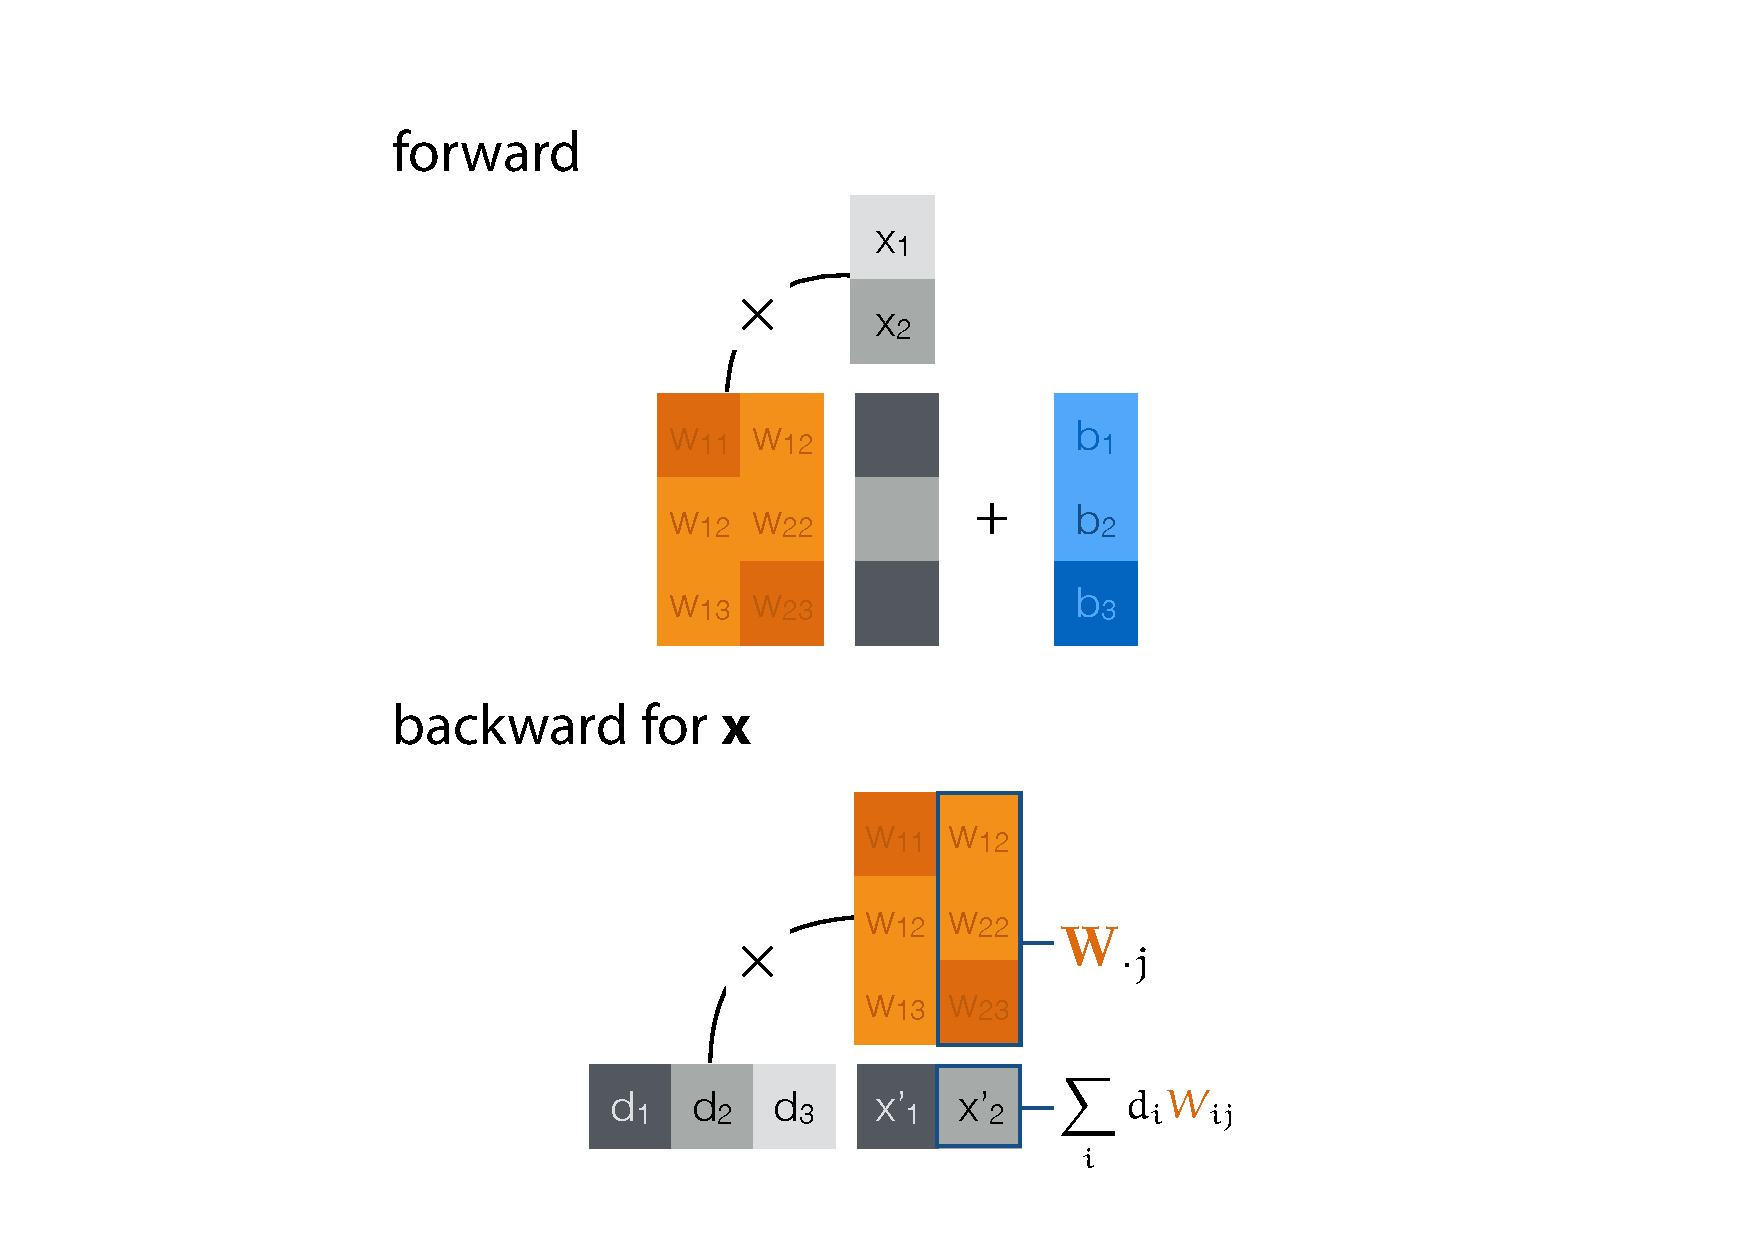
\includegraphics[width=0.7\linewidth]{matbp}

}{}

\section{Bonus: Expectation Maximization}

\emph{This is not an exam question, but it's helpful to do if you want to understand the EM algorithm.}

Assume we have a Gaussian Mixture Model in one dimension with two components: $\rc{N(0, 1)}$ and $\gc{N(1,1)}$. The weights $\rc{w_1}$ and $\gc{w_2}$ of the components are equal. 

{
\centering
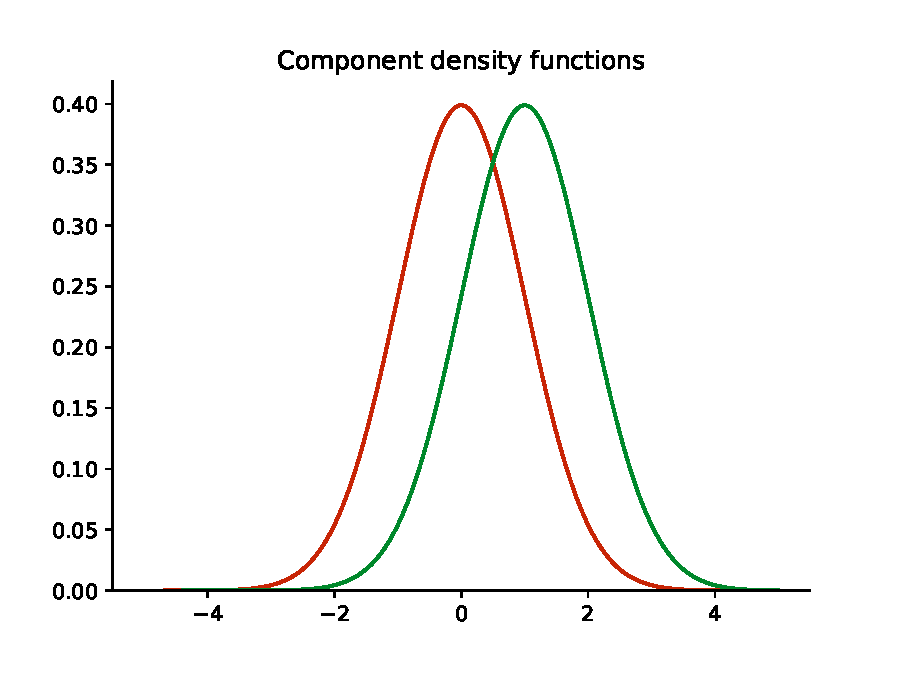
\includegraphics[width=0.7\linewidth]{hw-components-unscaled} \\
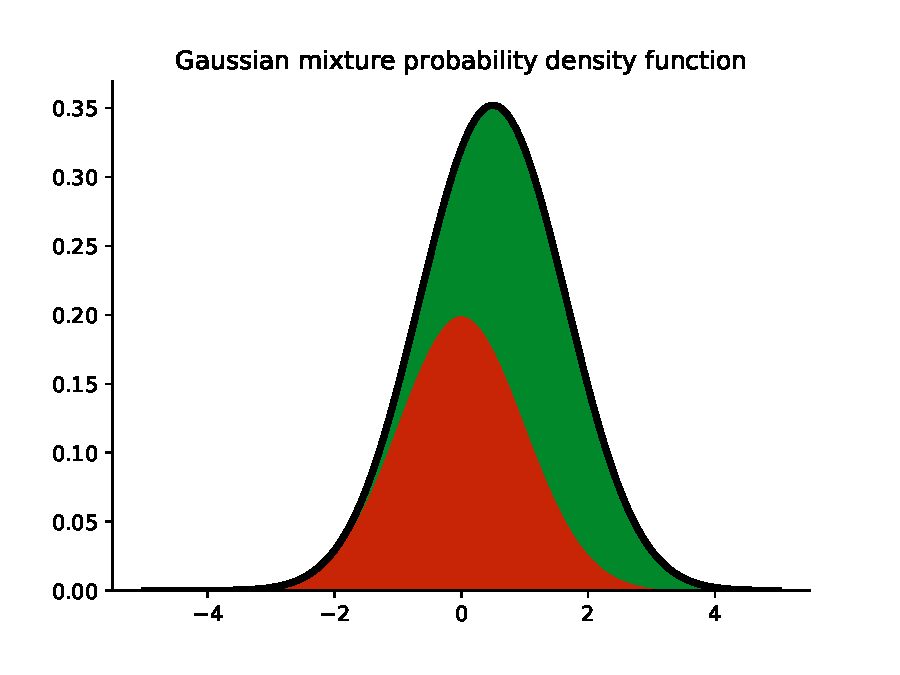
\includegraphics[width=0.7\linewidth]{hw-stackplot}
}

\qu Compute the probability density of the point 0, under the Gaussian Mixture.
\ans{
\begin{align*}
p(0) &= \rc{\frac{1}{2} N(0, 1)} + \gc{\frac{1}{2} N(1,1)}\\
 &= \rc{\frac{1}{2\sqrt{2\pi}} \exp(0)} + \gc{\frac{1}{2\sqrt{2\pi}} \exp\left(-\frac{1}{2}\right)} \\
 &= \rc{\frac{1}{2}\frac{1}{\sqrt{2 \pi}}} + \gc{\frac{1}{2}\frac{1}{\sqrt{2 \pi e}}} \approx 0.32
\end{align*}
}{}

\qu Under the EM algorithm, what responsibility is assigned to each component for the point 0?

\ans{
To compute the responsibility, we compute the probability of the component $z$ given the point $x$: $p(z\mid x)$, and normalize over all components. 
We get for component 1:
\[
\frac{\rc{\frac{1}{2\sqrt{2\pi}} \exp(0)}}{\rc{\frac{1}{2\sqrt{2\pi}} \exp(0)} + \gc{\frac{1}{2\sqrt{2\pi}} \exp\left(-\frac{1}{2}\right)}} = \frac{\rc{1}}{\rc{1} + \gc{\frac{1}{\sqrt{e}}}} \approx 0.62
\]
and for component 2: 
\[
\frac{\gc{\frac{1}{2\sqrt{2\pi}} \exp\left(-\frac{1}{2}\right)}}{\rc{\frac{1}{2\sqrt{2\pi}} \exp(0)} + \gc{\frac{1}{2\sqrt{2\pi}} \exp\left(-\frac{1}{2}\right)}} = \frac{\gc{\frac{1}{\sqrt{e}}}}{\rc{1} + \gc{\frac{1}{\sqrt{e}}}} \approx 0.37
\]

Note: Using Bayes' rule, this translates to $p(z\mid x) = \frac{p(x\mid z)p(z)}{p(x)}$. The denominator is the sum computed in the previous exercise, and the responsibilities are the proportions of each term to the total.\footnotemark

This is no accident, it is essentially what Bayes' rule tells us: to compute $p(z\mid x)$, we find $p(x)$ by marginalizing $Z$ out of $p(X=x, Z)$. This gives us a big sum, with one term for each $z$. The proportion of this term to the total is $p(z\mid x)$.

}{}

\end{document}